 \section{FURTHER OPTIMIZATION BY V\textsubscript{TH} ASSIGNMENT}
\label{sec:TVA}
% (1)
In the section, V\textsubscript{th} assignment is introduced to manipulate clock skew for aging tolerance. The idea comes from the aforementioned prior work~\cite{chen2013novel}, which exploits the technique to minimize the aging-induced clock skew, while it does not make the skew useful. Since V\textsubscript{th} assignment can also manipulate the clock skew, why do not we use the technique to achieve aging tolerance? We do. The two techniques,  V\textsubscript{th} assignment and aging manipulation are applied together to further optimize the required $T_c$. In other words, in addition to aging manipulation based on DCC insertion/deployment, we reassign the threshold voltage of certain clock buffers, such that the latencies of the buffers are changed, so are the slacks, which give us the opportunity to further mitigate the aging-induced degradation of logic network based on timing borrowing. The section is organized as follows:~\ref{sec:TVA:example} demonstrates how V\textsubscript{th} assignment further optimizes the required $T_c$.~\ref{sec:TVA:leader} introduces the rule/mechanism of V\textsubscript{th} assignment, followed by~\ref{sec:TVA:leaderconstraint}, which explains how we convert the rule/mechanism into CNF clauses.~\ref{sec:TVA:timingconstraint} introduces the new timing constraints when V\textsubscript{th} assignment is considered. Finally,~\ref{sec:TVA:experiment} shows the experimental results, which is optimized based on DCC insertion and V\textsubscript{th} assignment.

% (2)
%--------------------------------- Motivating Example -------------------------------------------------------
\subsection{Motivating Example considering V\textsubscript{th} assignment}
\label{sec:TVA:example}
We use the illustrative example to explain how we further improve the aging tolerance by comparing the two examples of Section~\ref{sec:motivate} and this section, based on the design in Figure~\ref{fig:sub:example}. The example in Section~\ref{sec:motivate} only considers the aging manipulation based on DCC deployment/insertion; however, in this section, the two approaches, DCC deployment and V\textsubscript{th} assignment are applied together to optimize/reduce required $T_c$. We let the DCC deployment same with that in the first example (in Section~\ref{sec:motivate}), i.e., 20\% DCC and 80\% DCC are inserted at the inputs of buffer 1 and buffer 2, respectively. Moreover, we begin reassigning high V\textsubscript{th} to the certain clock buffers, which are in the intervals from buffer 2 to \ce{FF_x} and  to \ce{FF_y}. In other words, buffer 2 and its downstream buffers are reassigned to high V\textsubscript{th}. To include the aging rates of HTV (High Threshold Voltage, or High-V\textsubscript{th}) buffers in the setup-time constraint, we assume that, the fresh/non-aging delay of HTV buffer is 1.2X longer than that of nominal buffer (whose V\textsubscript{th} are not reassigned), and aging rates of HTV buffer, with the duty cycle of 20\%, 40\%, 50\% and 80\%, are 0.5\%, 4.1\%, 5.4\% and 8.2\%, respectively. Note that, the aging rates of HTV buffer are lower than those of nominal buffer, because the higher/lower V\textsubscript{th} leads to lower/higher aging rates~\cite{chen2013novel}. Consider the new aging factors in the setup-time constraints on \ce{L_{XY}} and \ce{L_{YZ}}:
\begin{equation}
	\mbox{\fontsize{8}{9.6}\selectfont \ce{L_{XY}}:\quad$\textbf{1.09}C_X+1.2T_{cq}+1.15D_{XY}+1.2T_{su}<\textbf{(1.2+0.08)}C_Y+T_c$} 
	\label{eq:lxy2}
\end{equation}
\begin{equation}
	\centering
	\mbox{\fontsize{8}{9.6}\selectfont \ce{L_{YZ}}:\quad$\textbf{(1.2+0.08)}C_Y+1.2T_{cq}+1.15D_{YZ}+1.2T_{su}<\textbf{(1.2+0.08)}C_Z+T_c$} 
	\label{eq:lyz2}
\end{equation}
By re-arranging Equations (\ref{eq:lxy2}) and (\ref{eq:lyz2}):
\begin{flalign*}
	\hspace{1.2em}\ce{L_{XY}}: T_c &> 96.5 &\\
	\hspace{1.2em}\ce{L_{YZ}}: T_c &> 104
\end{flalign*}

Apparently, the required $T_c$ is further reduced/optimized from 108.5 (in Section~\ref{sec:motivate}) to 104 by inserting two DCCs and V\textsubscript{th} assignment in the existing synthesized clock network. We also observe that, the required $T_c$ is not dominated by \ce{L_{XY}} anymore (in Section~\ref{sec:motivate}); instead, it turns out that \ce{L_{YZ}} dominates $T_c$. As it can be seen, when the two approaches, V\textsubscript{th} assignment and aging manipulation  (by DCC insertion), are applied together, the skew for \ce{L_{XY}}, which equals 1.28$C_Y$ minus 1.09$C_X$, is larger than that in Section~\ref{sec:motivate}. Therefore, the new skew for \ce{L_{XY}} is more useful/beneficial and accounts for the better optimization of required $T_c$. 
Additionally, when it comes to the timing-borrowing mechanism of the two examples, there exists a difference: The timing-borrowing mechanism in Section~\ref{sec:motivate}, is achieved by the aging-induced clock skew, caused by manipulating the duty-cycle delivered to flip-flops. However, in the example, the timing-borrowing mechanism is based on aging-induced clock skew and \textit{tech-induced} clock skew, which is caused by manipulating the technology of clock buffers, i.e., reassign the V\textsubscript{th} of clock buffers. 

%--------------------------------- Leader -------------------------------------------------------
\subsection{Technology Leader}
\label{sec:TVA:leader}
When V\textsubscript{th} assignment is considered, how to select shortlisted clock buffers arises as a problem. The so-called shortlisted buffers are those whose V\textsubscript{th} will be reassigned (i.e., their technology is changed). Because the count and the combination of shortlisted buffers are numerous, we need to reduce the complexity of the problem. Thus, we introduce the rule of V\textsubscript{th} assignment by explaining \textit{technology leader}. 

If the clock buffer is chosen as the \textit{technology leader}, the clock buffer and its downstream buffers are regarded as shortlisted buffers. In other words, the technology of the buffer and the downstream buffers will be replaced with new counterpart. For example, in~\ref{sec:TVA:example}, buffer 2 is actually chosen as the technology leader, so that the shortlisted buffers are buffer 2 and its downstream buffers, which also include buffer 3. Note that, there is a difference between DCC and technology leader. DCC is not a clock buffer but a special-purpose gate, which is inserted at the input of the clock buffer, such that the aging rates of downstream buffers are manipulated; however, technology leader is an existing clock buffer. More specifically, it is selected from the buffers in the existing clock tree and indicates where we begin manipulating the technology of downstream buffers toward flip-flops.

% (4)
%--------------------------------- Framework -------------------------------------------------------
\subsection{Proposed Framework considering V\textsubscript{th} Assignment}
\label{sec:TVA:framework}
\begin{figure}
	\centering
	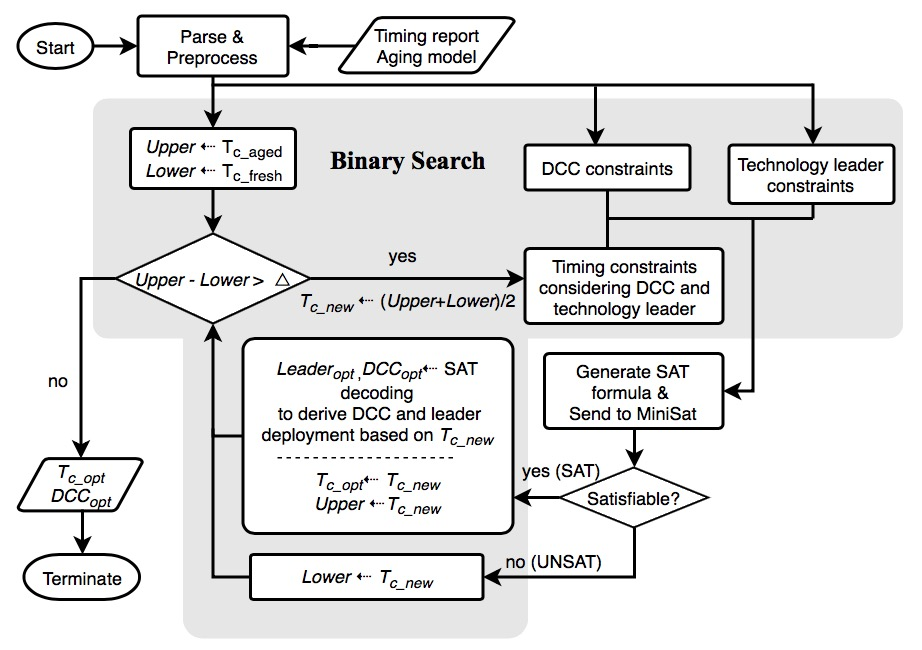
\includegraphics[width=0.9\columnwidth]{Flow_chart_tva.png}
	\caption{The overall flow of the framework when technology leaders are considered }
	\label{fig:flow:tva}
\end{figure}
The proposed framework, which considers aging manipulation (DCC) and V\textsubscript{th} assignment (technology leader), is depicted in Figure~\ref{fig:flow:tva}. Compared with the leader-free framework in Figure~\ref{fig:flow}, it is also based on a binary search for the minimum clock period ($T_c$) and SAT formulation. The problem, technology leader selection from clock buffers, is formulated as SAT problem, so is the problem of DCC insertion/deployment. In the sequel, Section~\ref{sec:TVA:leader_encode} explains how the problem of DCC insertion and technology leader selection is encoded by Boolean variables. Section~\ref{sec:TVA:leaderconstraint} introduces technology leader constraints, which is similar to DCC constraint. Section~\ref{sec:TVA:leaderconstraint} introduces the timing constraints which consider DCC deployment and technology leader selection. Finally,  Section~\ref{sec:TVA:leaderconstraint} shows the further optimized experimental results, based on DCC deployment and technology leader selection.

%--------------------------------- Encoding -------------------------------------------------------
% (5)
\subsection{Encoding for DCC and Technology Leader Deployment}
\label{sec:TVA:leader_encode}
The problem of DCC deployment and technology leader selection needs to be encoded into Boolean representation before being transformed into a SAT-based formulation. Assume that a total of $N$ types of DCCs can be chosen. Including the DCC-free case where no DCC is inserted, there are ($N$ + 1) possibilities of DCC insertion for each clock buffer. Furthermore, we also assume that a total of $M$ types of technology leaders can be chosen. Note that, each type of technology leader represents an individual technology. Including the nominal technology, there are ($M$ + 1) possibilities of technology leader selection for each clock buffer. We denote a clock buffer by $p\left(1 \leq p \leq P\right)$ where $P$ is the number of buffers. For each clock buffer, there exist two types of Boolean variables, $B_{p,q}$ and $B_{p,r}$, where $1 \leq p \leq P$, $1 \leq q \leq Q \leq r \leq R$, $Q = \lceil \lg (N + 1)\rceil$ and $R = \lceil \lg \{(N + 1)(M + 1\}\rceil$. $B_{p,q}$ are used to encode the ($N$ + 1) possibilities of DCC insertion, and $B_{p,r}$ are used to encode the ($M$ + 1) possibilities of technology leader selection.


\begin{figure}
    \centering
    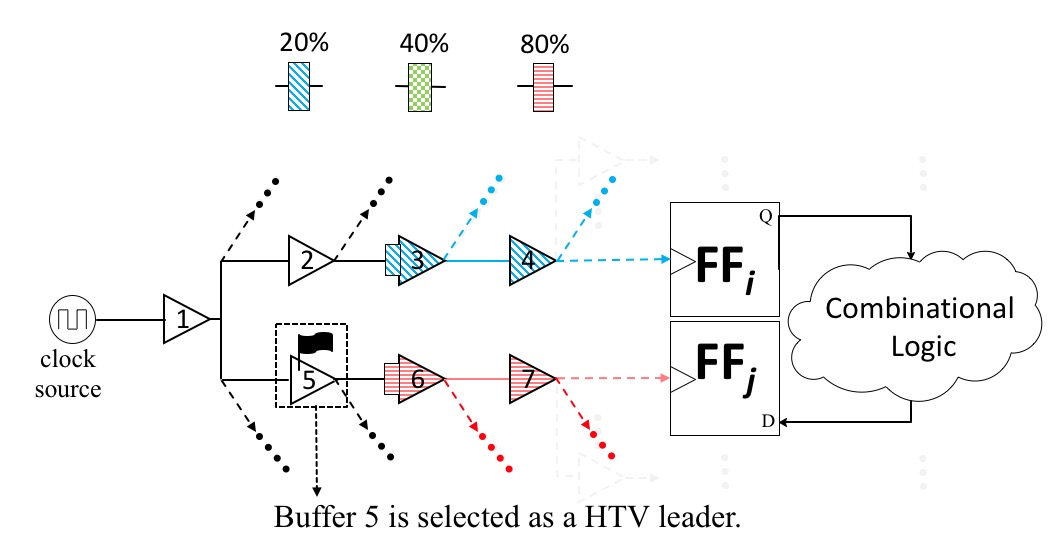
\includegraphics[width=0.9\columnwidth]{example_of_dcc_leader.png}
    \caption{An example with DCC deployment and technology selection}
    \label{fig:example_dcc_tva}
\end{figure}

Without loss of generality, we assume $N$ = 3, and $M$ = 1. Thus, there are three types of DCCs, which are assumed to be 20\%, 40\%, and 80\% DCCs, as shown in Figure~\ref{fig:dcctype}. In addition, there is one type of technology leader, which is assumed to be a HTV (high threshold voltage or high-V\textsubscript{th}) leader. Note that, if the clock buffer is selected as the HTV leader, the technology of the buffer and the associated downstream ones is replaced with high-V\textsubscript{th} counterpart. Since we assume three types of DCC and one type of technology leader, three Boolean variables are used for encoding eight possibilities of DCC and technology leader at any buffer. The eight possibilities can be encoded as follows:

\begin{tabular}{  c  c  c  c  }
  	 & Leader type & DCC type & $\{B_{p,3}, B_{p,2}, B_{p,1}\}$ \\ 
  	(1)\quad & Nominal V\textsubscript{th} & None & \{0, 0, 0\} \\ 
  	(2)\quad & Nominal V\textsubscript{th} &20\% &  \{0, 0, 1\} \\ 
  	(3)\quad & Nominal V\textsubscript{th} &40\% &  \{0, 1, 0\} \\ 
  	(4)\quad & Nominal V\textsubscript{th} &80\% &  \{0, 1, 1\} \\ 
	(5)\quad & HTV & None & \{1, 0, 0\} \\ 
  	(6)\quad & HTV & 20\% &  \{1, 0, 1\} \\ 
  	(7)\quad & HTV & 40\% &  \{1, 1, 0\} \\ 
  	(8)\quad & HTV & 80\% &  \{1, 1, 1\} \\ 
\end{tabular}


For example, in Figure~\ref{fig:example_dcc_tva}, the DCC deployment is same with that in Figure~\ref{fig:sub:dcci2} (i.e., 20\% DCC at buffer 3 and 80\% DCC at buffer 6), but the buffer 5 is selected as the HTV leader, which is denoted by a black flag. Thus, the technology of buffer 5, 6 and 7 are replaced with the high-V\textsubscript{th} counterpart. Therefore, $\left\{B_{3,3}, B_{3,2}, B_{3,1}\right\}$ = \{0, 0, 1\}, $\left\{B_{5,3}, B_{5,2}, B_{5,1}\right\}$ = \{1, 0, 0\}, $\left\{B_{6,3}, B_{6,2}, B_{6,1}\right\}$ = \{0, 1, 1\}, and $\left\{B_{p,3}, B_{p,2}, B_{p,1}\right\}$ = \{0, 0, 0\} for $p$ = 1, 2, 4 or 7.

As mentioned in Section~\ref{subsec:eddcd}, the 20\% DCC mitigates the aging of buffer 3 and its downstream buffers, but the 80\% DCC aggravates the aging of buffer 6 and its downstream buffers. Moreover, since the buffer 5 is a HTV leader, buffer 5, 6 and 7 are changed as high-V\textsubscript{th} buffers, implying the latency from buffer 5 to buffer 7 is lengthened. This way, the clock skew becomes larger than that in Figure~\ref{fig:sub:dcci2}, so that the required $T_c$ can be further reduced, based on timing borrowing. Note that, as we mentioned in Section~\ref{sec:TVA:example}, the $T_c$ reduction in Figure~\ref{fig:sub:dcci2} is only due to the useful aging-induced clock skew; however, the  further $T_c$ reduction in Figure~\ref{fig:example_dcc_tva} is both based on useful aging-induced and tech-induced clock skew, which is caused by the V\textsubscript{th} reassignment of clock buffers. 
% (6)

%--------------------------------- Constraints - Preface -------------------------------------------------------
\subsection{Constraints and Corresponding Clauses}
\label{sec:TVA:leaderconstraint}
\begin{figure}
    \centering
    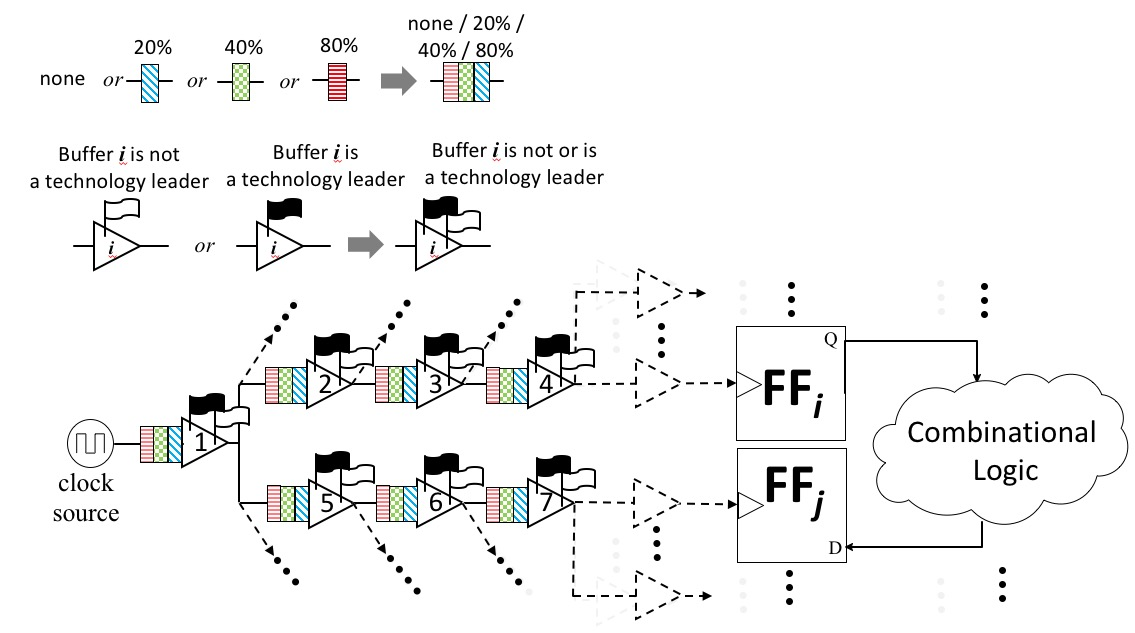
\includegraphics[width=1\columnwidth]{All_types_of_DCCs_and_leaders.png}
    \caption{Generalized DCC insertion and technology leader selection for a target pair of flip-flops}
    \label{fig:g_dcc_leader}
\end{figure}

Figure~\ref{fig:g_dcc_leader} shows a generalized example of DCC insertion and technology leader selection for a pair of flip-flops (\ce{FF_i} and \ce{FF_j}), where there exist aging-critical paths from \ce{FF_i} to \ce{FF_j}. As described in Section~\ref{subsec:dccccc}, a path is defined as an aging-critical path if it is possible to determine the clock period of the circuit, in the presence of aging. Each pair of flip-flops between which there exist aging-critical paths needs to be considered. Here, we use the generalized example to illustrate our SAT-based formulation. The generalized example in Figure~\ref{fig:g_dcc_leader} is similar to that in Figure~\ref{fig:dcctype}. In contrast, we include technology leader selection for each clock buffer in Figure~\ref{fig:g_dcc_leader}. Moreover, we can find that, if the clock buffer, which is selected as a technology leader, is deep in the clock tree (i.e., close to flip-flops), the count of V\textsubscript{th}-reassigned buffers is reduced thus the impact of tech-induced clock skew becomes insignificant. The above phenomenon is similar to that in Section ~\ref{subsec:eddcd}, which observes that deeper DCC deployment causes less aging-induced clock skew. Thus, we set a rule of avoiding selecting/inserting leaders/DCCs at a clock tree level, which is larger/deeper than a specified boundary.  The rule greatly reduce the complexity of SAT-based formulation, because a significant fraction of buffers are not considered being inserted DCC at their inputs and being selected as a technology leader. For instance, in Figure~\ref{fig:g_dcc_leader}, dashed buffers and their downstream buffers are not considered. 

In Figure~\ref{fig:g_dcc_leader}, buffers 1 - 7 are candidate locations for DCC insertion and leader selection. According the encoding mechanism explained in Section~\ref{sec:TVA:leader_encode}, one Boolean variables are introduced to encode the two possibilities of leader selection, for each of the seven buffers. Thus, there are totally 128 (=$2^7$) possibilities of leader selection, only for this pair of flip-flops. In contrast, there is a total of 16,384 (= $4^7$) possibilities of DCC  deployment. If we combine the two approaches (i.e., DCC insertion and leader selection) together, there is totally 2,097,152 possibilities. The total count of possibilities can be obtained by multiplying the possibilities of the two approaches (i.e., $4^7*2^7$ = 2,097,152), or can be explained by the eight possibilities of DCC insertion and leader selection, for each of the seven buffers (i.e., $8^7$ = 2,097,152). Apparently, this make SAT-based formulation tricky because of clause explosion. Therefore, we set the following constraints on DCC insertion and technology leader selection.

%--------------------------------- DCC Constraints -------------------------------------------------------
% (7)
\subsubsection{DCC Constraints and Corresponding Clauses}
\label{sec:TVA:dcc_c}
The DCC constraints are identical to those in Section~\ref{subsec:dccccc}. That is, at most one DCC exists along a single clock path, from clock source to one of flip-flops. The corresponding clauses can be referred to the 48 clauses in Section~\ref{subsec:dccccc}. After applying DCC constraints, the total possibilities of DCC insertion can be reduced from 16,384 (= $4^7$) to 103. 

%--------------------------------- Tech Leader Constraints -----------------------------------------------
% (8)
\subsubsection{Technology Leader Constraints and Corresponding Clauses}
\label{sec:TVA:dcc_c}
The leader constraints are similar to DCC constraints. They are defined as follow: At most one technology leader exists along a single clock path, from clock source to one of the flip-flops. To ensure no more than one leader along any clock path, we can use the Boolean variables, which are introduced to encode leader selection, i.e., $B_{p,r}$, where $1 \leq p \leq P$, $\lceil \lg \{(N + 1)\} \rceil = Q \leq r \leq R = \lceil \lg \{(N + 1)(M + 1)\} \rceil$, to generate some clauses which suppress the occurrence of having two leaders along a clock path. Consider buffer 2 (encoded by $\left\{B_{2,3}\right\}$) and buffer 3 (encoded by $\left\{B_{3,3}\right\}$) in Figure~\ref{fig:g_dcc_leader}. If buffer 2 is a leader (i.e., $\{B_{2,3}\} \not\equiv \{0\}$), then buffer 3 must not be a leader (i.e., $\{B_{3,3}\} \equiv \{0, 0\}$), and vice versa. The constraint can be formally written as:
\begin{gather*}
\left(\{B_{2,3}\} \equiv \{0\}\right) \lor \left(\{B_{3,3}\} \equiv \{0, 0\}\right)
\end{gather*}
Next, it can be translated into one CNF clause:
\begin{gather*}
\mbox{\fontsize{7}{8.4}\selectfont ($\neg B_{2,3}\lor\neg B_{3,3}$) )} 
\end{gather*}

Any pair of buffers along a single clock path should be constrained in this way. Among buffers 1 $\hyphen$ 7 in Figure~\ref{fig:dcctype}, there are 12 pairs: $\langle1, 2\rangle$, $\langle1, 3\rangle$, $\langle1, 4\rangle$, $\langle1, 5\rangle$, $\langle1, 6\rangle$, $\langle1, 7\rangle$, $\langle2, 3\rangle$, $\langle2, 4\rangle$, $\langle3, 4\rangle$, $\langle5, 6\rangle$, $\langle5, 7\rangle$, $\langle6, 7\rangle$. Each pair translates to one clause and a total of 12 clauses will be generated accordingly.

With leader constraints and corresponding clauses, we can drastically reduce the possibilities of leader selection to be formulated. In the above example where 12 clauses associated with leader constraints are generated, when we only consider the possibilities of leader selection, the count drops from 128 (= $2^7$) to 17. Furthermore, when DCC deployment are included, and DCC constraints and leader constraints are applied together, the possibility count drops from 2,097,152 to 1751. In the next subsection, we describe what the 17 and 1751 possibilities are and how they are translated into final CNF representation.

%--------------------------------- Timing Constraints (DCC+TVA) - Preface -----------------------------------------------
% (9)
\subsection{Timing Constraints considering DCC and Technology Leader}
\label{sec:TVA:timingconstraint}
\begin{figure*}
    \centering
    \subfigure[Case 2-1: One leader on the common clock path (e.g., at buffer 1), and two DCCs]{
    	\label{fig:sub:dccleaderi1}
        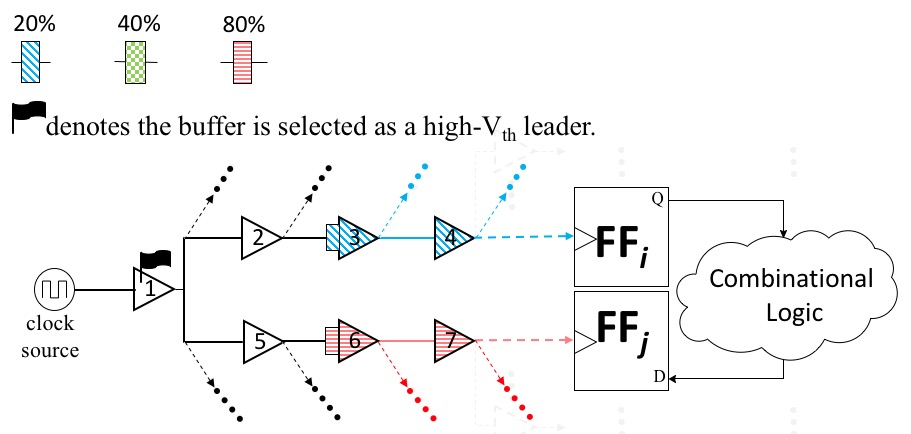
\includegraphics[width=0.9\columnwidth]{2DCC_1Leader.png}
    }
    \hspace{1cm}
    \subfigure[Case 2-2: one leader on one of the divergent clock paths, or class 3: two leaders, one on each of the divergent clock paths]{
    	\label{fig:sub:dccleaderi2}
        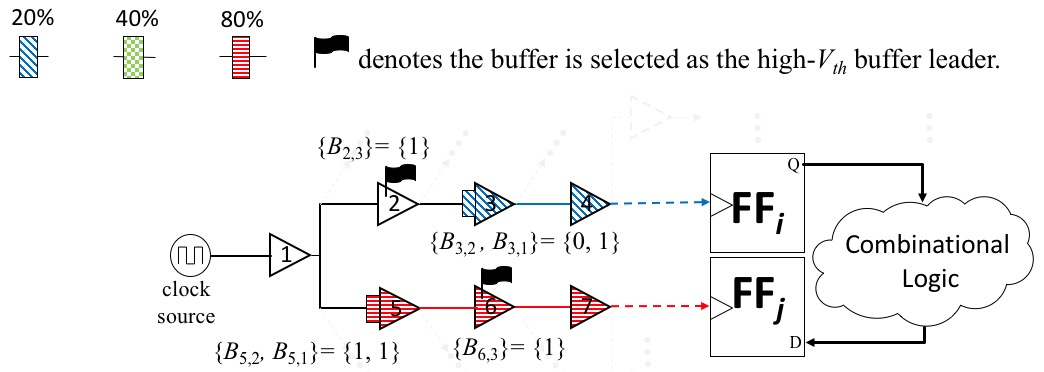
\includegraphics[width=0.9\columnwidth]{2DCC_2Leader.png}
    }
    \caption{Examples of DCC insertion}
    \label{fig:dccleaderinsert}
\end{figure*}
The timing constraints, considering the two approaches, is extended from those in Section~\ref{subsec:tccc}. As seen in Section~\ref{subsec:tccc}, given a pair of flip-flops, between which there exists one logic path, the timing (i.e., setup-time and hold-time) constraints must be met based on the inequalities~(\ref{eq:tsu}) and~(\ref{eq:th}). The previous timing constraints in Section~\ref{subsec:tccc} only consider the aging influence on clock latency, with the DCC deployment in the clock tree. Thus, the new timing constraints in the subsection need to include the influence of V\textsubscript{th} reassignment on clock latency. 

Given one clock period $T_c$ derived by binary search, one aging-critical logic path, and its associated clock network, the previous timing constraints are classified into 3 classes, according to the used DCC count (i.e., no, one, and two DCC insertions). The new timing constraints are extended from the 3 classes, each of which are further classified into 3 subclasses, according to the leader count (i.e., the count of buffers which are selected as leaders). Thus, there are totally 9 (= $3*3$) subclasses based on the count of DCC and leader. For brevity, 6 of the 9 subclasses are omitted in the following discussion. We only discuss the other 3 subclasses, whose DCC deployment is given identically, but leader counts vary from 0, 1 to 2. Furthermore, due to the aforementioned DCC and leader constraints, the SAT solver will only output a DCC/leader deployment/selection where there does not exist more than one DCC/leader along any clock path. Thus, in the following discussion, the deployment with more than one DCC/leader along a single clock path can be ignored. In each subclass, if the DCC deployment and leader selection cause a timing violation within 10 years (i.e., the lifespan specification), then the deployment/selection will be transformed into CNF clauses, such that the solver will not output the deployment/selection as results. Here, we explain the generation of CNF clauses by using the example in Figure~\ref{fig:dccleaderinsert}.

%--------------------------------- Timing Constraints (DCC+TVA) - Class 1 -----------------------------------------------
\setcounter{class}{0}
\begin{class}
\label{class:c4}
No buffer on either clock path is selected as a technology leader

Consider the situation that, among buffers 1 $\hyphen$ 7, no buffer is selected as a technology leader. If it causes a timing violation along the aging-critical path within 10 years, then the Boolean representation of the deployment,
\begin{gather*}
\left(\{B_{1,3}, B_{1,2}, B_{1,1}\} \equiv \{0, 0, 0\} \right) 
\land \left( \{B_{2,3}, B_{2,2}, B_{2,1}\} \equiv \{0, 0, 0\} \right) \\ \land \dotsb 
\land \left( \{B_{7,3}, B_{7,2}, B_{7,1}\} \equiv \{0, 0, 0\} \right),
\end{gather*}
equivalent to the following CNF clause:
\begin{gather*}
(B_{1,3} \lor B_{1,2} \lor B_{1,1} \lor B_{2,3} \lor B_{2,2} \lor B_{2,1} \\ \lor \dotsb \lor B_{7,2} \lor B_{7,2} \lor B_{7,1} ),
\end{gather*}
should be generated such that the solver will not output the corresponding DCC deployment and leader selection in the result if the CNF is satisfiable. In this case, a total of 1 CNF clause is generated.
\end{class}

%--------------------------------- Timing Constraints (DCC+TVA) - Class 2 -----------------------------------------------
\begin{class}
\label{class:c5}
Only one buffer is selected as a technology leader

This class can be further classified into 2 sub-classes based on the buffer location of technology leader. \\
\textit{Class 2-1:} Selected buffer (i.e., technology leader) on the common clock path.

In Figure~\ref{fig:dccleaderinsert}, buffer 1 is on the common clock path. Consider the leader selection shown in Figure~\ref{fig:sub:dccleaderi1}: if buffer 1 is the HTV leader and the leader selection causes a timing violation within 10 years, then the Boolean representation of the leader selection and the DCC deployment, $\left(\{B_{1,3}, B_{1,2}, B_{1,1}\} \equiv \{1, 0, 0\} \right) \land \left( \{B_{2,3}, B_{2,2}, B_{2,1}\} \equiv \{0, 0, 0\} \right) \land \left( \{B_{3,3}, B_{3,2}, B_{2,1}\} \equiv \{0, 1, 0\} \right) \land \left( \{B_{4,3}, B_{4,2}, B_{4,1}\} \equiv \{0, 0, 0\} \right) \land \left( \{B_{5,3}, B_{5,2}, B_{5,1}\} \equiv \{0, 0, 0\} \right) \land  \left( \{B_{6,3}, B_{6,2}, B_{6,1}\} \equiv \{0, 1, 1\} \right) \land \left( \{B_{7,3}, B_{7,2}, B_{7,1}\} \equiv \{0, 0, 0\} \right)$, equivalent to the following clause: 
$(\neg B_{1,3} \lor B_{1,2} \lor B_{1,1} \lor B_{2,3} \lor B_{2,2} \lor B_{2,1} \lor B_{3,3} \lor \neg B_{3,2} \lor B_{3,1} \\ 
\lor B_{4,3} \lor B_{4,2} \lor B_{4,1} \lor B_{5,3} \lor B_{5,2} \lor B_{5,1} \lor B_{6,3} \lor \neg B_{6,2} \lor B_{6,1} \\ 
\lor B_{7,3} \lor B_{7,2} \lor B_{7,1} )$, should be generated such that the solver will not output the leader selection and DCC deployment in the result if the CNF is satisfiable. Given that there are 1 choices of technology leader, a total of 1 CNF clause will be generated in the worst case. \\

%DATE 2018
%if the insertion of a 40\% DCC at buffer 1 causes a timing violation within 10 years, then the Boolean representation of the DCC deployment, $\left(\{B_{1,2}, B_{1,1}\} \equiv \{1, 0\} \right) \land \left( \{B_{2,2}, B_{2,1}\} \equiv \{0, 0\} \right) \land \dotsb \land \left( \{B_{7,2}, B_{7,1}\} \equiv \{0, 0\} \right)$, equivalent to the following clause: $\left(\neg B_{1,2} \lor B_{1,1} \lor B_{2,2} \lor B_{2,1} \lor \dotsb \lor B_{7,2} \lor B_{7,1} \right)$, should be generated such that the solver will not output the deployment in the result if the CNF is satisfiable. Given that there are 3 choices of DCCs, a total of 3 CNF clauses will be generated in the worst case. \\

%\textit{Class 2-2:} \mbox{\fontsize{9}{10.8}\selectfont Selected buffer (i.e., technology leader) is on one of the divergent clock paths}
\textit{Class 2-2:} Selected buffer (i.e., technology leader) is on one of the divergent clock paths.

This class targets buffers 2, 3, 4, 5, 6, 7. If buffer 2 is the HTV leader, and it causes a timing violation within 10 years, then the Boolean representation of the leader selection and the DCC deployment, $\left(\{B_{2,3}, B_{2,2}, B_{2,1}\} \equiv \{1, 0, 0\} \right) \land \left( \{B_{1,3}, B_{1,2}, B_{1,1}\} \equiv \{0, 0, 0\} \right) \land \left( \{B_{3,3}, B_{3,2}, B_{3,1}\} \equiv \{0, 1, 0\} \right) \land \left( \{B_{4,3}, B_{4,2}, B_{4,1}\} \equiv \{0, 0, 0\} \right) \land \left( \{B_{5,3}, B_{5,2}, B_{5,1}\} \equiv \{0, 0, 0\} \right) \land \left( \{B_{6,3}, B_{6,2}, B_{6,1}\} \equiv \{0, 1, 1\} \right) \land \left( \{B_{7,3}, B_{7,2}, B_{7,1}\} \equiv \{0, 0, 0\} \right)$, equivalent to the following CNF clause: 
$(B_{1,3} \lor B_{1,2} \lor B_{1,1} \lor \neg B_{2,3} \lor B_{2,2} \lor B_{2,1} \lor B_{3,3} \lor \neg B_{3,2} \lor B_{3,1} \lor B_{4,3} \lor B_{4,2} \lor B_{4,1} \lor B_{5,3} \\
\lor B_{5,2} \lor B_{5,1} \lor B_{6,3} \lor \neg B_{6,2} \lor  \neg B_{6,1} \lor B_{7,3} \lor B_{7,2} \lor B_{7,1} )$, should be generated such that the solver will not output the leader selection and DCC deployment in the result if the CNF is satisfiable. This class includes 6 candidates: buffers 2, 3, 4, 5, 6, 7, and each has 1 choice of technology leader. Therefore, a total of 6 CNF clauses will be generated in the worst case.
%DATE 2018
%This class targets buffers 2, 3, 4, 5, 6, 7. If the insertion of a 20\% DCC at buffer 3 causes a timing violation within 10 years, then the Boolean representation of the DCC deployment, $\left(\{B_{3,2}, B_{3,1}\} \equiv \{0, 1\} \right) \land \left( \{B_{1,2}, B_{1,1}\} \equiv \{0, 0\} \right) \land \dotsb \land \left( \{B_{7,2}, B_{7,1}\} \equiv \{0, 0\} \right)$, equivalent to the following CNF clause: $\left(B_{3,2} \lor \neg B_{3,1} \lor B_{1,2} \lor B_{1,1} \lor B_{2,2} \lor B_{2,1} \lor \dotsb \lor B_{7,2} \lor B_{7,1} \right)$, should be generated such that the solver will not output the deployment in the result if the CNF is satisfiable. This class includes 6 candidates: buffers 2, 3, 4, 5, 6, 7, and each has 3 choices of DCCs. Therefore, a total of 18 CNF clauses will be generated in the worst case.
\end{class}
%--------------------------------- Timing Constraints (DCC+TVA) - Class 3 -----------------------------------------------
\begin{class}
\label{class:c6}
Two buffers on two divergent clock paths are selected as technology leaders.

Given the DCC deployment and leader selection in Figure~\ref{fig:sub:dccleaderi2} (a 20\% DCC inserted at buffer 3, a 80\% DCC inserted at buffer 6, and buffer 2 and 5 are both  HTV leaders), if it causes a timing violation along the aging-critical path within 10 years, then the Boolean representation of the deployment, $\left(\{B_{1,3}, B_{1,2}, B_{1,1}\} \equiv \{0, 0, 0\} \right) \land \left( \{B_{2,3}, B_{2,2}, B_{2,1}\} \equiv \{1, 0, 0\} \right) \land \left( \{B_{3,3}, B_{3,2}, B_{3,1}\} \equiv \{0, 1, 0\} \right) \land \left( \{B_{4,3}, B_{4,2}, B_{4,1}\} \equiv \{0, 0, 0\} \right) \land \left( \{B_{5,3}, B_{5,2}, B_{5,1}\} \equiv \{1, 0, 0\} \right) \land \left( \{B_{6,3}, B_{6,2}, B_{6,1}\} \equiv \{0, 1, 1\} \right) \land \left( \{B_{7,3}, B_{7,2}, B_{7,1}\} \equiv \{0, 0, 0\} \right)$, equivalent to the following  CNF clause: 
$(B_{1,3} \lor B_{1,2} \lor B_{1,1} \lor \neg B_{2,3} \lor B_{2,2} \lor B_{2,1} \lor B_{3,3} \lor \neg B_{3,2} \lor B_{3,1} \lor B_{4,3} \lor B_{4,2} \lor B_{4,1} \lor \neg B_{5,3} \\
\lor B_{5,2} \lor B_{5,1} \lor B_{6,3} \lor \neg B_{6,2} \lor  \neg B_{6,1} \lor B_{7,3} \lor B_{7,2} \lor B_{7,1} )$, should be generated such that the solver will not output the deployment in the result if the CNF is satisfiable.

Class 3 considers the selection of the two technology leaders, one among buffers \{2, 3, 4\} and the other one among buffers \{5, 6, 7\}; thus, there are totally 9 (=$3^2$) combinations of HTV leader selection. Therefore, a total of 9 CNF clauses will be generated in the worst case.

Considering all of the above cases with the given DCC deployment, a maximum number of 1 + 1 + 6 + 9 = 17 clauses can be derived. This is based on the existence of 12 clauses introduced in Section~\ref{sec:TVA:dcc_c}. If we consider the 103 combinations of DCC deployment in Section~\ref{subsec:tccc}, a total of 1751 (=$103*17$) clauses can be derived in the worst case.

\end{class}

%--------------------------------- Experimental Results ----------------------------------------------------------------
% (10)
\subsection{Experimental Results}
\label{sec:TVA:experiment}
The proposed framework, which simultaneously considers the two techniques, is implemented in C++ and SAT-based formulation is solved by MiniSat. The experimental environment and benchmark circuits are identical to the previous setting in Section~\ref{sec:exp}.
Under 10-year aging influence with BTI, the aging rates of clock buffers are obtained from HSPICE. The aging rates of nominal clock buffers with duty cycles of 20\%, 40\%, 50\%, and 80\% are 8.5\%, 12.1\%, 13.5\%, and 16.4\% respectively and the aging rate of logic is obtained by using the same predictive model. The timing information of HTV buffers is estimated from the model in~\cite{andres2016}. The fresh/non-aging delays of HTV buffers are 1.2X longer than that of nominal buffer, and the aging rates with duty cycle of 20\%, 40\%, 50\%, and 80\% are 0.5\%, 4.1\%, 5.4\%, and 8.2\%, respectively.


